\documentclass[../main/main.tex]{subfiles}

\begin{document}
\espacio

  En este capítulo se muestra en detalle la problemática de la investigación, la justificación del problema con una visión desde diferentes enfoques de acuerdo a los paradigmas tecnológico y científico, así como los alcances y límites de la investigación.

  \section{Planteamiento del problema}

  La CPU ejecuta las tareas que le son asignadas de acuerdo a una secuencia definida mediante criterios de prioridad o tiempos de llegada, estos procesos pueden ser a su vez pausados para resolver tareas con un mayor nivel de criticidad de acuerdo al algoritmo de planificación de colas que la CPU utilice; de esta manera, estas tareas ingresan a una cola de espera, que dependiendo del trabajo de la CPU, pueden tardar un tiempo considerable en ser atendidos, e inclusive desecharse por la excesiva carga de trabajo de la CPU. En las comunicaciones encriptadas, dada la lógica inherente de los procesos de encriptación, los tiempos de ejecución pueden llegar a incrementarse hasta un punto insostenible para un solo procesador, por lo cual los fabricantes, de acuerdo a las limitaciones de tamaño y frecuencia máxima de la CPU, vieron necesario el incremento del número de procesadores a fin de atender los procesos en la cola y evitar desechar tareas por los tiempos excesivos de ejecución.

  Para resolver este problema se plantea la alternativa de procesamiento descentralizado mediante la delegación de trabajos a la GPU; a su vez, se medirá la diferencia de tiempos mediante la comparación del tiempo de ejecución del Algoritmo de Encriptación Avanzada AES Rijndael ejecutado en la CPU versus el tiempo de ejecución del proceso en la GPU haciendo uso del entorno de programación Python, que cabe señalar, cuenta con compatibilidad nativa para la ejecución de tareas en matrices de procesadores CUDA mediante la librería Numba\footnote{\href{http://numba.pydata.org/numba-doc/latest/cuda/index.html}{NumPy+Mamba=Numba: Array-oriented Python Compiler for NumPy}}.

  \section{Justificación tecnológica}

  Como se mencionó anteriormente, de acuerdo al paradigma actual del desarrollo de hardware de microprocesadores, se llegó a un límite difícil de superar con los materiales de fabricación actuales.

  Intel propuso el modelo de desarrollo de hardware ``Tick-Tock'' que consiste en un lanzamiento cada 18 meses (1 año y medio), ambas palabras hacen referencia a:

  \begin{description}[noitemsep,nolistsep]
    \item[Tick:] Mejoría de una arquitectura anterior
    \item[Tock:] Lanzamiento de una nueva arquitectura
  \end{description}

  Pero si se realiza una comparación del último ``Tock'' que realizó Intel con respecto al microprocesador de la gama i7, se obtiene un resultado claro, y es que en 6 años se redujo el tamaño de transistor de 22nm a 14nm, duplicando los procesadores para llegar a un total de 8 procesadores físicos del CPU Intel i7-3770 del año 2012 al procesador Intel i9-9900 del año 2018. Pero la frecuencia se incrementó tan solo en 2MHz, por lo tanto se puede concluir que el paradigma tiene como objetivo llegar a multiplicar el número de procesadores pero no así la frecuencia de trabajo de los mismos.

  \begin{table}[H]
    \centering
    \caption{Comparación procesadores Intel i7}
    \begin{tabular}{|p{5.6cm}|p{4cm}|p{4cm}|}
  \hline
  \multicolumn{1}{|c|}{\textbf{Característica}} & \textbf{I9-9900K} & \textbf{I7-3770} \\ \hline
  Núcleos & 8 & 4 \\ \hline
  Hilos & 16 & 8 \\ \hline
  Serie & Coffee Lake & Ivy Bridge \\ \hline
  Socket & FCLGA1151 & FCLGA1155 \\ \hline
  Fecha de lanzamiento & 4º trimestre de 2018 & 2º trimestre de 2012 \\ \hline
  Cache & 16 MB & 8 MB \\ \hline
  Set de instrucciones & SSE4.1, SSE4.2, AVX2 & SSE4.1/4.2, AVX \\ \hline
  Litografía & 14 nm & 22 nm \\ \hline
  Velocidad de bus & 8 GT/s DMI3 & 5 GT/s DMI \\ \hline
  Solución térmica & PCG 2015D (130W) & 2011D \\ \hline
  Máximo tamaño de memoria & 64 GB & 32 GB \\ \hline
  Tipo de memoria & DDR4-2666 & DDR3 1333/1600 \\ \hline
  Ancho de banda de memoria & 41.6 GB/s & 25.6 GB/s \\ \hline
  Frecuencia base para gráficos & 350 MHz & 650 MHz \\ \hline
  Frecuencia máxima para gráficos & 1.20 GHz & 1.15 GHz \\ \hline
  Configuración de PCI Express & 1x16, 2x8, 1x8+2x4 & 1x16, 2x8, 1x8 \& 2x4 \\ \hline
\end{tabular}
    \caption*{\textbf{Fuente:} \href{https://cpu.userbenchmark.com/Compare/Intel-Core-i9-9900K-vs-Intel-Core-i7-3770/4028vs1979}{\cite{web:i9_vs_i7}}}
  \end{table}

  Por lo tanto se justifica el uso de la Unidad de Procesamiento Gráfico para la distribución de tareas repetitivas aptas para un enfoque de ejecución en paralelo, ya que de acuerdo a la tabla comparativa anterior se observa que el paradigma de desarrollo de hardware por parte de los fabricantes es hacia un ecosistema de procesadores en paralelo en lugar de un bajo número de procesadores trabajando a frecuencias altas.

  \section{Justificación científica}

  En lo referente al ámbito científico, la utilidad de esta investigación radica en la profundización del estudio acerca de los métodos de ejecución de aplicaciones en múltiples hilos utilizando la Unidad de Procesamiento Gráfico (GPU), con la finalidad de llegar a utilizar las mallas de procesadores disponibles en las tarjetas gráficas, este estudio a la fecha de realización de la presente investigación, aún no se ha profundizado, ni es de aplicación general.

  Por tanto, al concluir esta investigación, se habrán aportado los resultados a la investigación de ejecución de tareas en paralelo en la GPU que podrán ser utilizados como base para otros métodos de encriptación u otros procesos no necesariamente relacionados con criptografía.

  \section{Alcances y límites} \label{limites_alcances}

  El algoritmo utilizado y modificado para la obtención de resultados en CPU y GPU, cumple con la definición de la Publicación de Estándares de Procesamiento de Información Federal 197\footnote{Federal Information Processing Standards Publications - FIPS 197}. [\cite{report:FIPS_197}]. Dicha publicación fue aprobada por el Instituto Nacional de Estándares y Tecnología\footnote{National Institute of Standards and Technology - NIST} después de la verificación en la Reforma de Administración de Tecnologías de la Información\footnote{Information Technology Management Reform} de 1996.

  El relleno de datos de 128 bits cumple con el Estándar de Criptografía de Llave Pública PKCS \#7 plasmado en el reporte RFC 2315 [\cite{report:RFC_2315}].

  \begin{figure}[H]
    \centering
    \caption{Microprocesador Intel i7-3770}
    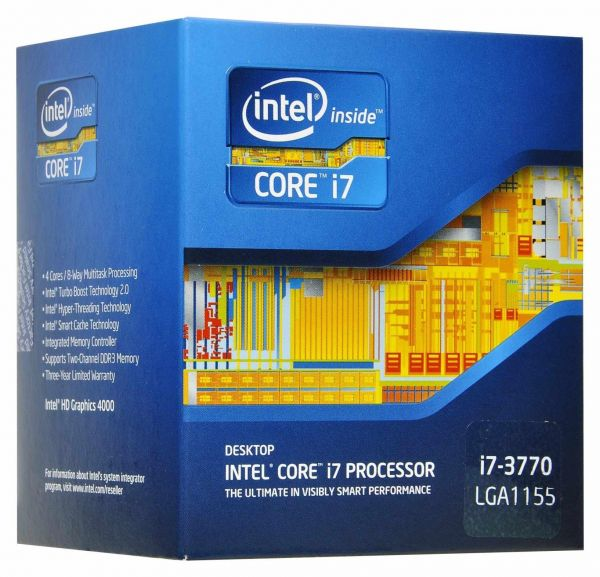
\includegraphics[width=7cm, keepaspectratio]{problema/intel_i7.jpg}
    \caption*{\textbf{Fuente:} \href{https://tinyurl.com/yb3tqpvu}{Intel® Core™ i7-3770 Processor, ark.intel.com}}
  \end{figure}

  En cuanto al hardware, se realiza la comparación de tiempo de ejecución en el microprocesador Intel i7-3770\footnote{\href{https://tinyurl.com/yb3tqpvu}{Intel® Core™ i7-3770 Processor, ark.intel.com}} con respecto a la tarjeta gráfica NVidia GTX 650 Ti\footnote{\href{https://tinyurl.com/ycr3kouv}{NVidia GeForce GTX-650Ti, www.geforce.com}}. Lo que representa una comparativa de trabajo simultáneo de 8 núcleos trabajando a 3.4GHz versus 768 núcleos trabajando a 928MHz para las operaciones pasibles a paralelismo.

  El algoritmo, modificado para esta investigación, fue escrito originalmente por Pablo Caro y es de código abierto, se puede encontrar en la plataforma Github\footnote{\href{https://github.com/pcaro90/Python-AES}{Python-AES, Pablo Caro}}. El código original no cuenta con ninguna ejecución de procesos en paralelo.

  \begin{figure}[H]
    \centering
    \caption{Tarjeta Gráfica NVidia GeForce GTX-650Ti}
    
\includegraphics[width=12cm, keepaspectratio]{problema/gtx_650ti.png}
    \caption*{\textbf{Fuente:} \href{https://tinyurl.com/ycr3kouv}{NVidia GeForce GTX-650Ti, www.geforce.com}}
  \end{figure}

  Se realizaron modificaciones al algoritmo mencionado anteriormente mediante la librería Numba que cuenta con decoradores predefinidos que compilan el código para que pueda ser paralelizado. Esta librería genera kernels compatibles con plataformas CUDA de distintas arquitecturas.

  El sistema operativo utilizado para la investigación es Arch Linux con el Kernel versión 4.18.10.

  El driver de NVidia que se utilizó es de la versión 410.57-2 con el manejador de procesadores CUDA versión 10.0.130-2.

  La versión de Python utilizada fue 3.6.7, con las librerías externas Numba v0.41 y Numpy v1.15.1.
\end{document}